\documentclass[dvipdfmx,a4]{jsarticle}
\usepackage{amsmath,amssymb}
\usepackage{mathtools,amssymb}
\usepackage{bm}
\usepackage{ascmac}
\usepackage{graphicx}
\usepackage[dvipdfmx]{color}
\usepackage{tikz}
\usepackage[version=4]{mhchem}
\usepackage{xcolor}
\usepackage{here}
\usepackage{wrapfig}
\usetikzlibrary{intersections,calc,arrows.meta}

\title{斜交座標を使おう}
\author{中越一磨}
\begin{document}
\maketitle

\section{直交座標系の線形代数的表示}
斜交座標系の話題を始める前に,直交座標系について考え直してみる.直交座標系で3つの軸に沿った単位ベクトルを\(\vec{e_x}\),\(\vec{e_y}\),\(\vec{e_z}\)定義したとき,空間内任意の点Pは\(\vec{p}=(x,y,z)\)という表し方とは別に\(\vec{p}=x\vec{e_x} + y\vec{e_y} +z\vec{e_z}\)という,基底ベクトルの線型結合の形で表現することもできる.基底ベクトルとは,ここでは単に座標軸を決めるような単位ベクトルくらいの理解で良い.また,線型結合はベクトルを和で結合しいるだけである.

今回用いた3つの基底ベクトルは具体的には\(\vec{e_x}=(1,0,0)\),\(\vec{e_y}=(0,1,0)\),\(\vec{e_z}=(0,0,1)\)と定義してる.それぞれのベクトルの内積は直交しているのだから,
\begin{equation*}
  \vec{e_i}\cdot \vec{e_j} = \delta_{ij}
\end{equation*}
である.ただし\(i,j=x,y,z\)\footnote{以後,\(x,y,z\)のうような明示的なインデックスを振らないことがあるので注意してほしい.}であり,\(\delta_{ij}\)はKroneckerのデルタであり\(i=j\)となるときは1で,\(i\not =j\)のときに0となるようなものである.以後このような表示は便利なので用いる.

\section{直交座標系以外の軸のとり方は許されないのか}
これまでは,座標系といえば直交座標系であったであろう.直交座標系とは,文字通り座標軸がそれぞれ直交関係にあるような座標系であり普通に考えれば,便利なものであるし特殊な場合を考えない限りは直交座標系で事足りるであろう.

\begin{figure}[htbp]
  \centering
  \begin{minipage}{0.3\columnwidth}
    \centering
    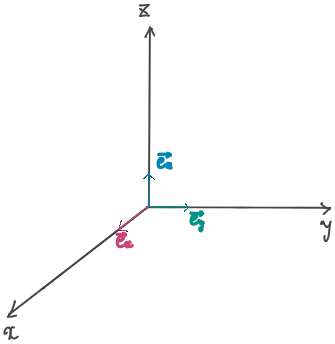
\includegraphics[width=\columnwidth]{fig/cartecian.pdf}
    \caption{直交座標系}
    \label{car}
  \end{minipage}
  \begin{minipage}{0.25\columnwidth}
    \centering
    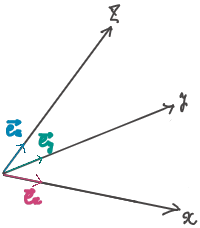
\includegraphics[width=\columnwidth]{fig/oblique.pdf}
    \caption{斜交座標系}
    \label{obl}
  \end{minipage}
\end{figure}

しかし,場合によっては直交座標系で考えるより見通しがあるようなものがあるだろう.例えば,高校数学Bにおいての空間図形を扱う際,基準となるベクトル(基底ベクトル)は必ずしも直交していない場合は多々あるであろう.むしろ直行していない状況のほうが多いであろう.

一つ具体例について考えよう.図\ref{fig1}のような正四面体は例題として頻出である.このような対称を扱う際に,基準のベクトルは基本的には頂点の一つを原点としてその点からの延びる3本の辺に沿ってベクトルを\(\vec{a}(=\overrightarrow{OA})\),\(\vec{b}(=\overrightarrow{OB})\),\(\vec{c}(=\overrightarrow{OC})\)と設定するのが素直であろう.このとき,この3つの基準のベクトルはもちろん直交していない.ただし,この先のことも考えてそれぞれのベクトルは単位ベクトル\footnote{単に大きさが1のベクトルのこと.}であるとする.


\begin{figure}[tbh]
  \centering
  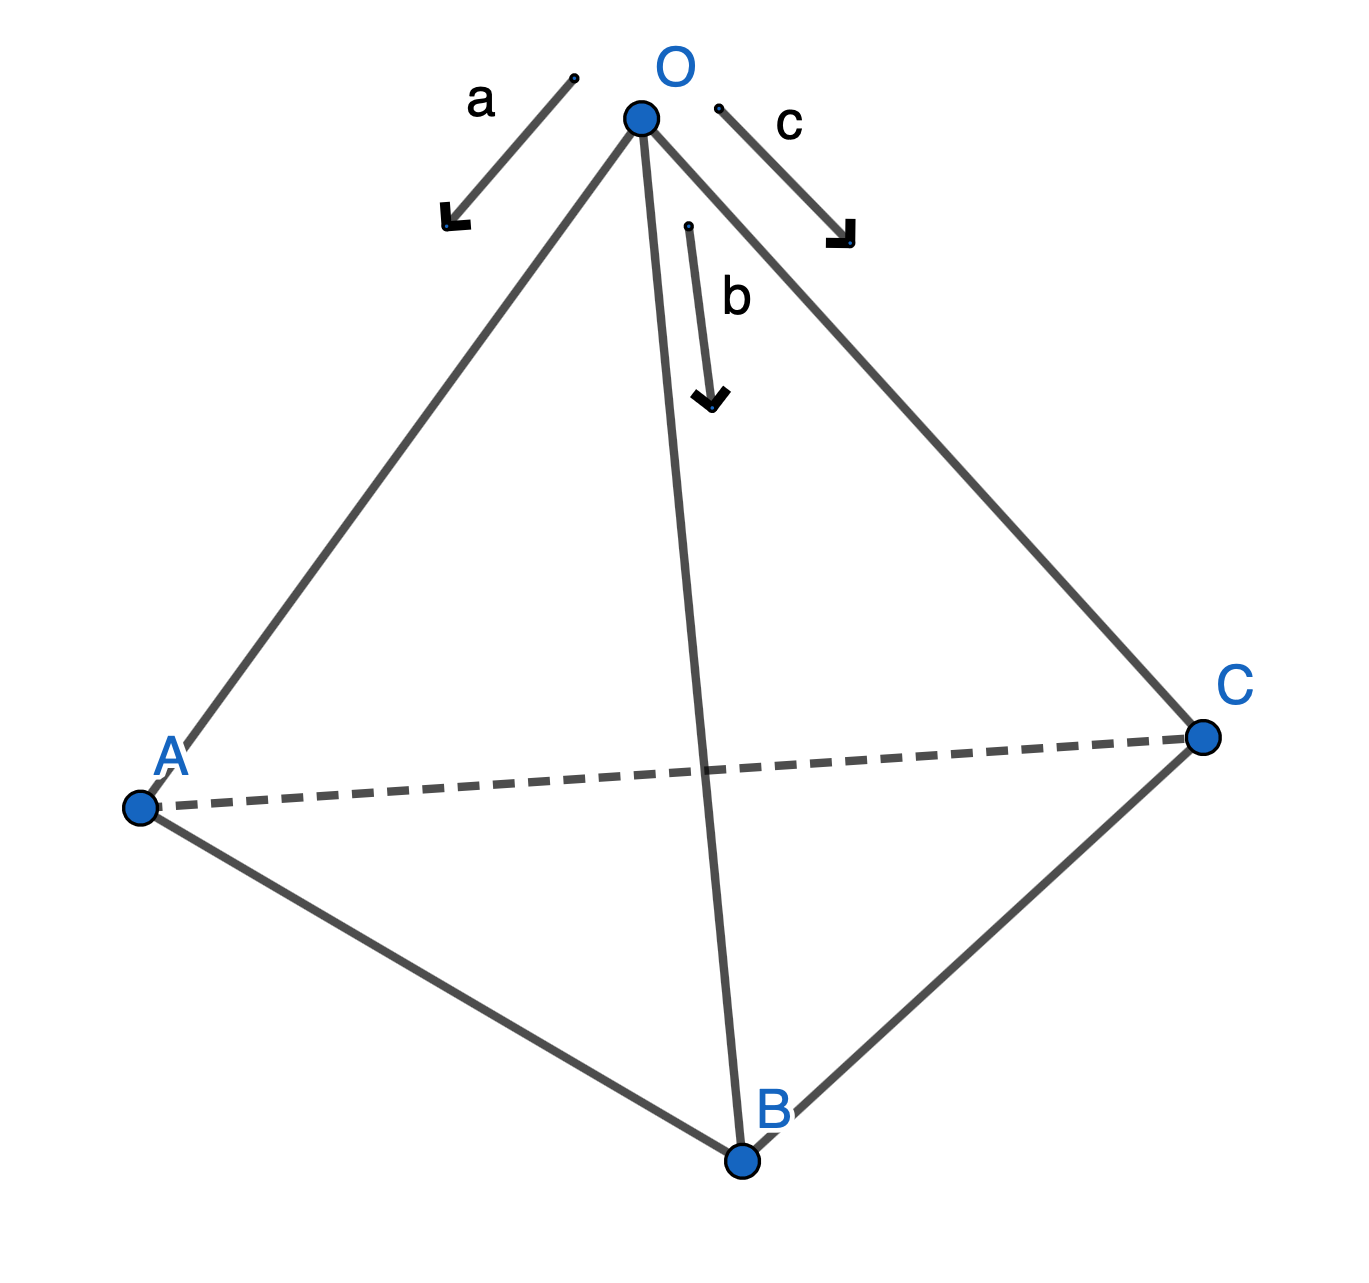
\includegraphics[height=6cm]{fig/fig1.png}
  \caption{正四面体}
  \label{fig1}
\end{figure}

このような状況下で,この正四面体内の各点をこれらの3つのベクトルで表していき問題を解いていくことは,ある程度空間ベクトルの問題に取り組んできた者であれば理解できると思う.例えば,この正四面体の重心\(\vec{g}\)は
\begin{equation*}
  \vec{g} = \dfrac{1}{3}\left( \vec{a}+\vec{b}+\vec{c} \right)
\end{equation*}
で表せる.ここで1.で考えた表示のアイデアを借りれば,これら3つのベクトルの組を基底ベクトルとしてそれらを実数倍にして線形結合した座標のような表示が可能であるということが容易に想像できると思う.具体的に,ある空間中の点P(\(\vec{p}\))に対して
\begin{equation*}
  \vec{p} = a \vec{a} + b \vec{b} +c \vec{c}
\end{equation*}
のように表示することができ,直交座標系のときのようにそれぞれの基底を\(\vec{a}=(1,0,0)\),\(\vec{b}=(0,1,0)\),\(\vec{c}=(0,0,1)\)のように定義すれば,\(\vec{p} =(a,b,c)\)のように座標のように扱うことができる.

しかしここで問題になるのは計算規則は直交座標系のときと同じように扱ってよいのかということである.結論を先に述べるとだめである.斜交座標がしっかりと使えるよう次の項でしっかりと定義していこう.

\section{斜交座標}
\subsection{斜交座標の問題点}
この問題によって引き起こされることは任意の2つのベクトルの内積を考えたとき,顕著に現れる.今,2次元平面を斜交座標をとったときの基底ベクトルを\(\vec{e_1}\),\(\vec{e_2}\)として2つのベクトル\(\vec{v_1} = a\vec{e_1} +b\vec{e_2}\),\(\vec{v_2} = c\vec{e_1} +d\vec{e_2}\)として,内積を考えると
\begin{eqnarray}
  \vec{v_1}\cdot \vec{v_2}
  &=& \left( a\vec{e_1} +b\vec{e_2} \right)\cdot \left( c\vec{e_1} +d\vec{e_2} \right)\\
  &=& ac \, \vec{e_1} \cdot \vec{e_1} + ad\, \vec{e_1} \cdot \vec{e_2} +\cdot bc\, \vec{e_2} \cdot \vec{e_1} +bd\, \vec{e_2} \cdot \vec{e_2} \label{2}
\end{eqnarray}
のようになる.式(2)を見るとわかるように,第1項と第4項のみを考えれば直交座標系での内積と同じである.しかし,今斜交座標系では第2項,第3項のようないわゆる非対角項\footnote{この言葉の意味は後にわかる.}がゼロになる保証などなにもない.なぜなら,\(\vec{e_1} \cdot \vec{e_2} \neq 0\)であるためである.それゆえに,直交座標系のときのように内積を
\begin{eqnarray}
  \vec{v_1} \cdot \vec{v_2} \not=
  \begin{pmatrix}
    a \\
    b
  \end{pmatrix}
  \cdot
  \begin{pmatrix}
    c \\
    d
  \end{pmatrix}
  = ac+bd
\end{eqnarray}
のような計算を定義してもこれは誤りである.成分計算をうまく定義するにはどうしたら良いだろう,その表現のために行列について触れる.

\subsection{行列とその計算規則}
行列は,はじめに聞いても何がしたいのかがよくわからないと思う.ここでは必要最低限の行列について触れる.行列の存在意義や考える意味などについては一概には言えないが,物理数学の観点から見ればベクトルの拡張,ベクトルに変換を施すものなどというような目的をやんわりと理解してもらえれば差し付けないであろう.

行列とは,\(m\)行と\(n\)列のに方向に成分を持つ数の集まりである.例えば2行2列の行列は次のようになる.
\begin{equation*}
  \begin{pmatrix}
    1 & 2 \\
    3 & 4
  \end{pmatrix}
\end{equation*}
このような,ベクトルが一方向にのみに成分を持っていたような数の集まりであったことを拡張して,2次元的な拡張を行ったものが行列である.一般に行列\(A\)は次のように添字\(i,j\)の2つを用いて表す.
\begin{equation*}
  A= (a_{ij})=
  \begin{pmatrix}
    a_{11} & \cdots & a_{1j} & \cdots & a_{1n} \\
    \vdots & \ddots &        &        & \vdots \\
    a_{i1} &        & a_{ij} &        & a_{in} \\
    \vdots &        &        & \ddots & \vdots \\
    a_{n1} & \cdots & a_{nj} & \cdots & a_{nn}
  \end{pmatrix}
\end{equation*}
以降,行列は,行方向と列方向の成分数が等しいような正方行列のみについて記していく.2つの\(n\times n\)行列\(A=(a_{ij})\),\(B=(b_{ij})\)を定義して話をすすめる.
\subsubsection{行列の和}
行列の和は,それぞれの成分同士を足し合わせれば良い.なので,
\begin{equation*}
  A+B= (a_{ij}+b_{ij})=
  \begin{pmatrix}
    a_{11} +b_{11} & \cdots & a_{1j}+b_{1j}  & \cdots & a_{1n}+b_{1n} \\
    \vdots         & \ddots &                &        & \vdots        \\
    a_{i1} +b_{i1} &        & a_{ij} +b_{ij} &        & a_{in}+b_{in} \\
    \vdots         &        &                & \ddots & \vdots        \\
    a_{n1} +b_{n1} & \cdots & a_{nj} +b_{nj} & \cdots & a_{nn}+b_{nn}
  \end{pmatrix}
\end{equation*}
のようになる.

\subsubsection{行列の積}
行列の積は少々複雑な形をしている.\(n\times n\)行列同士の積の結果は\(n\times n\)行列であり,\(n\times m\)行列のような成分数の異なる者については\(n\times m\)と\(m\times l\)のように前後の列の成分数と行の成分数が一致するような場合にしか積は定義されていない.この定義からも予想できるように行列の積は一般に可換ではない.

では,行列の積の具体的な定義についてであるが,積\(AB\)によって生成される新たな行列の\(ij\)成分が前の行列の\(i\)行成分と後の行列の\(j\)列成分のそれぞれの積の総和をとったものになるようになっている.
\begin{equation}
  AB = \left (\sum ^n _{k=1} a_{ik}b_{kj} \right )_{ij}
  \label{e-matpro}
\end{equation}

\begin{figure}[tbh]
  \centering
  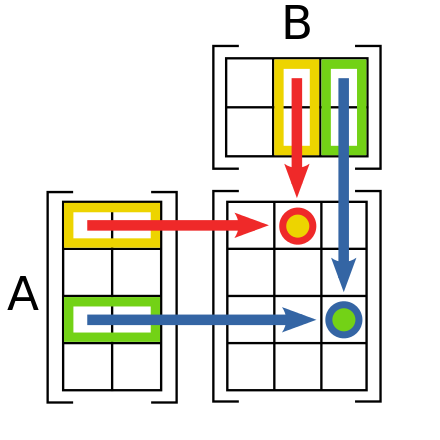
\includegraphics[height=5cm]{fig/matpro.png}
  \caption{行列の積のイメージ}
  \label{matpro}
\end{figure}
この定義から明らかなように,\(AB \neq BA\)である.また,積について結合則と分配則は成り立っている.証明は各自行ってほしい.最後に,行列の積における1のような役割を果たす単位行列について触れる.単位行列とは,\(i=j\)となるようなとき\footnote{このような成分を対角成分といい,それ以外の部分を非対角項と呼ぶ.}は1でそれ以外が0になるような行列でありEなどと表す.具体的には
\begin{equation*}
  E=
  \begin{pmatrix}
    1      & \cdots & 0 & \cdots & 0      \\
    \vdots & \ddots &   &        & \vdots \\
    0      &        & 1 &        & 0      \\
    \vdots &        &   & \ddots & \vdots \\
    0      & \cdots & 0 & \cdots & 1
  \end{pmatrix}
\end{equation*}
のようなものである.これを用いると,
\begin{equation*}
  EA= AE =A
\end{equation*}
のようになる.\footnote{単位行列はこの性質から正方行列の積に対する群の単位元になる.その意味では正方行列全体の集合は環を成している.}

\subsubsection{行列とベクトルの積}
行列とベクトルの積であるが,縦ベクトルと1行n列の行列と考えれば式\ref{e-matpro}の特別な場合と考えればよいということは少し手を動かしてみればわかると思う.とりあえず今回計算することになる3次元の場合について記す.

\begin{equation*}
  \begin{pmatrix}
    a_{11} & a_{12} & a_{13} \\
    a_{21} & a_{22} & a_{23} \\
    a_{31} & a_{32} & a_{33}
  \end{pmatrix}
  \begin{pmatrix}
    x \\
    y \\
    z
  \end{pmatrix}
  =
  \begin{pmatrix}
    a_{11}x + a_{12} y +a_{13}z \\
    a_{21}x + a_{22} y +a_{23}z \\
    a_{31}x + a_{32} y +a_{33}z \\
  \end{pmatrix}
\end{equation*}

\subsection{計量テンソル}
さて,行列についての定義・演算を終え準備は整ったので本題に戻りたい.式\refeq{2}を斜交座標を撮ったときの成分表示と行列で表現し直すと,
\begin{equation*}
  \vec{v_1}\cdot \vec{v_2}=
  \begin{pmatrix}
    a & b
  \end{pmatrix}
  \begin{pmatrix}
    \vec{e_1} \cdot \vec{e_1} & \vec{e_1} \cdot \vec{e_2} \\
    \vec{e_2} \cdot \vec{e_1} & \vec{e_2} \cdot \vec{e_2}
  \end{pmatrix}
  \begin{pmatrix}
    c \\
    d
  \end{pmatrix}
\end{equation*}
のようになる.これが基底直行しない場合での内積の定義の拡張になっている.では,この間に入っている行列の意味について考えよう.

直交座標のときが斜交座標の特別な場合であると考えると基底が直交するときはもとの内積になる必要がある.つまりはこの行列が単位行列になればよいということになる.一方で,基底が直交関係にあるときは非対角項は当然0となりこの条件を満たす.つまり,いままでは無視してよかった非対角項が斜交座標のようなより一般の座標では0とならないためその効果が生きてくるということがわかる.このように,この行列は座標系ないしは空間の性質を顕著に定める量となっているということがわかる.このような行列を計量テンソル\footnote{テンソルという言葉自体は今はそれほど大事ではないので割愛するが,ここでは行列と思っていて良い.ただ,テンソルは必ずしも行列として表されるものではないということには注意してほしい.また本当はより深い意味をもっていることには留意してほしい.}といい一般に\(g_{ij}\)と表記する.またその定義については,
\begin{equation*}
  (g_{ij}) = \begin{pmatrix}
    \vec{e_i} \cdot \vec{e_j}
  \end{pmatrix}
\end{equation*}
のようにしても問題ないように見えるが,内積の定義に内積を用いてしまっている点は少しいただけない部分である.しかし,斜交座標などのような場合についてのみであれば実用上は問題ないので今回はこれ以上踏み込まないこととする.

このような計量テンソルを用いて内積を再定義する.用いるベクトルは\(\vec{a} = (a_i)\),\(\vec{b} = (b_i)\)とする.
\begin{equation*}
  \vec{a}\cdot \vec{b}=
  \sum ^n _{i=1} \sum ^n _{j=1} g_{ij} a_{i} b_{j}
\end{equation*}
ここで,便利な記法を紹介する.同一項内に同じ添字が現れたらその添字について1からnまですべての和を取るというルールのもと和の記号を省略するというものである.これはEinsteinの縮約記法\footnote{Einsteinはこれを自身の数学における最大の発明と自称していた.}という.なので先程の式は
\begin{equation*}
  \vec{a}\cdot \vec{b}=  g_{ij} a_{i} b_{j}
\end{equation*}
という非常にシンプルなものとなる.

ちなみになぜ計量とという名がついているかについてだが,ベクトルの大きさについて考えたとき,
\begin{equation*}
  |a|^2 = \vec{a}\cdot \vec{a}=  g_{ij} a_{i} a_{j}
\end{equation*}
となり,距離に定めるための量であるという意味で計量と呼ばれる.

\section{具体例}
最後に,斜交座標系を用いて具体的な入試問題\footnote{この問題は神戸大学2018年文系に出題された数学の第1問を改題したものである.}に取り組んでみよう.

[問題]1辺の長さ1の正四面体\(OABC\)に対して,図\ref{fig2}のように,点Pは辺\(OA\)を\(t:1-t\)に内分した点であり,点Qは辺\(OB\)を\(1-t:t\)に内分した点であり,点Rは辺\(OC\)を\(1:1\)に内分した点である.このとき,三角形\(PQR\)の面積が最小となるような\(t\)とその面積を求めよ.
\begin{figure}[tbh]
  \centering
  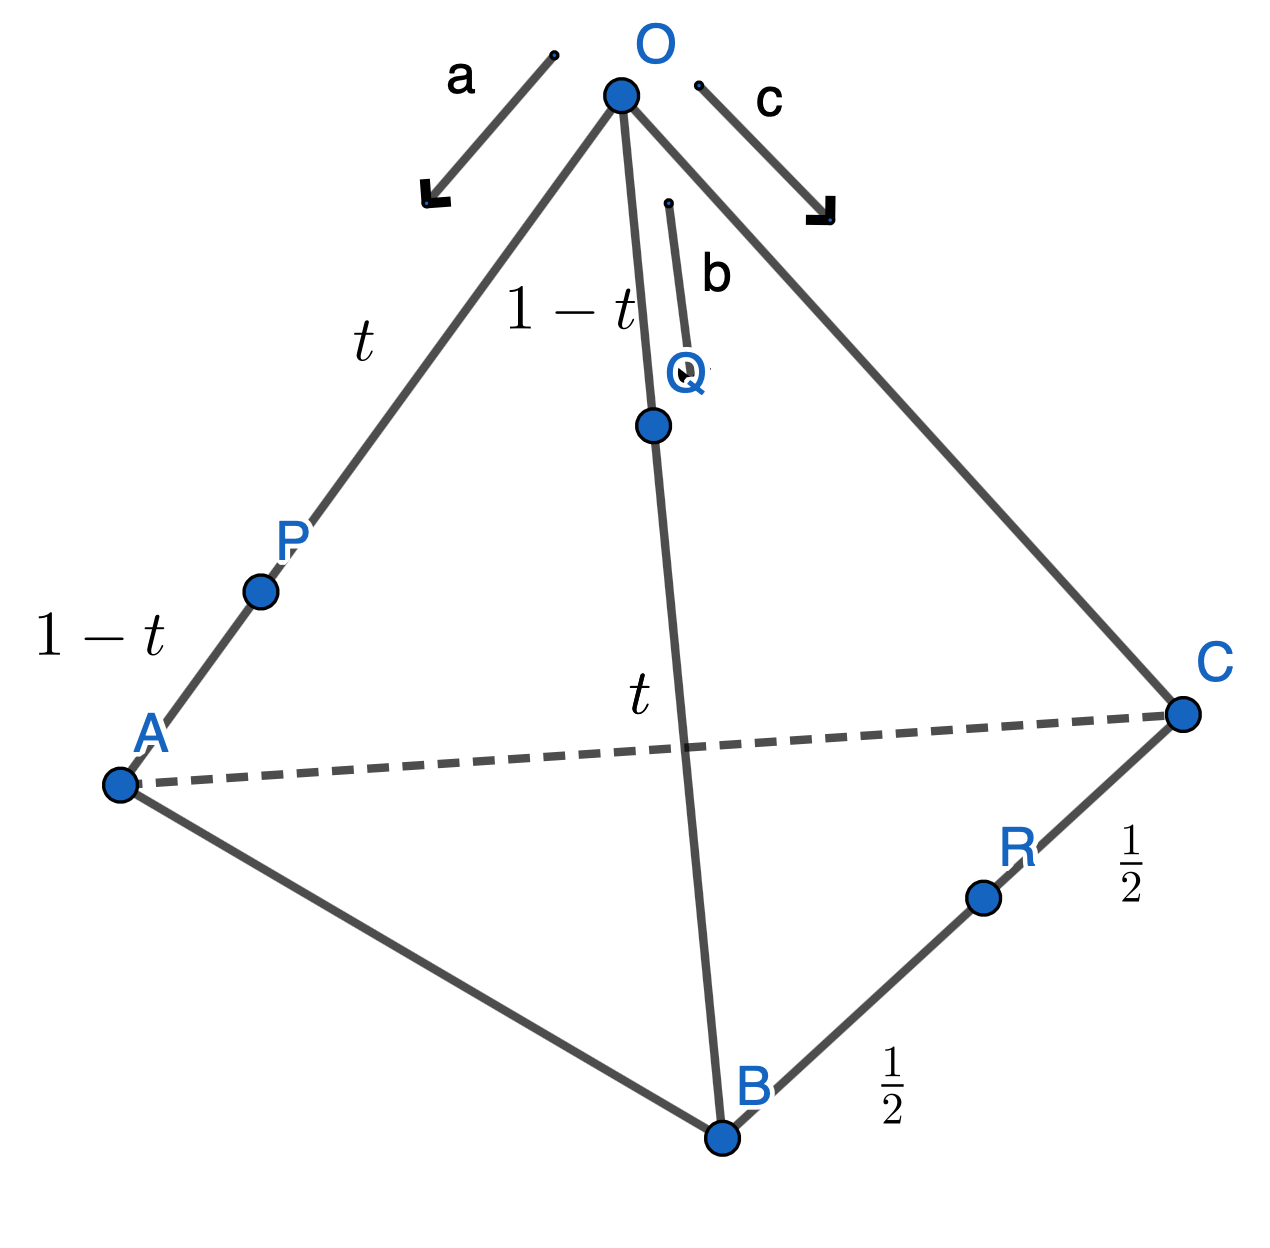
\includegraphics[height=5cm]{fig/fig2.png}
  \caption{正四面体の問題}
  \label{fig2}
\end{figure}

[解]
基底ベクトルを図のようにとったとき,点P,Q,Rを斜交座標で表したとき\((t,0,0)\),\((0,1-t,0)\),\((0,1/2,1/2)\)のようになる.また,計量テンソルは\(\vec{a}\cdot \vec{b}=\vec{b}\cdot \vec{c}=\vec{c}\cdot \vec{a}=1\cdot 1\cos \left( \dfrac{\pi}{3} \right) = \dfrac{1}{2} \)より
\begin{equation*}
  g_{ij}=
  \begin{pmatrix}
    1   & 1/2 & 1/2 \\
    1/2 & 1   & 1/2 \\
    1/2 & 1/2 & 1
  \end{pmatrix}
\end{equation*}
となる.\(\overrightarrow{QP} = (t, t-1, 0)\),\(\overrightarrow{QR} = (0, t-1/2, 1/2)\)なので,
ここでそれぞれの大きさは,
\begin{eqnarray*}
  |\overrightarrow{QP}| ^2
  &=&
  \begin{pmatrix}
    t & t-1 & 0
  \end{pmatrix}
  \begin{pmatrix}
    1   & 1/2 & 1/2 \\
    1/2 & 1   & 1/2 \\
    1/2 & 1/2 & 1
  \end{pmatrix}
  \begin{pmatrix}
    t   \\
    t-1 \\
    0
  \end{pmatrix}\\
  &=&
  (t+(t-1)/2)t+(t-1)(t/2+t-1)\\
  &=&
  3t^2 -3t +1
\end{eqnarray*}

\begin{eqnarray*}
  |\overrightarrow{QR}| ^2
  &=&
  \begin{pmatrix}
    0 & t-1/2 & 1/2
  \end{pmatrix}
  \begin{pmatrix}
    1   & 1/2 & 1/2 \\
    1/2 & 1   & 1/2 \\
    1/2 & 1/2 & 1
  \end{pmatrix}
  \begin{pmatrix}
    0     \\
    t-1/2 \\
    1/2
  \end{pmatrix}\\
  &=&
  t^2-\dfrac{1}{2}t+\dfrac{1}{4}
\end{eqnarray*}

また,\(\angle PQR=\theta\)は内積の定義式と成分計算を用いて
\begin{eqnarray*}
  \overrightarrow{QP}\cdot \overrightarrow{QR}
  &=&
  |\overrightarrow{QP}||\overrightarrow{QR}| \cos(\theta)\\
  &=&
  \begin{pmatrix}
    t & t-1 & 0
  \end{pmatrix}
  \begin{pmatrix}
    1   & 1/2 & 1/2 \\
    1/2 & 1   & 1/2 \\
    1/2 & 1/2 & 1
  \end{pmatrix}
  \begin{pmatrix}
    0     \\
    t-1/2 \\
    1/2
  \end{pmatrix}\\
  &=&
  \dfrac{3}{2}t^2-\dfrac{5}{4}t+\dfrac{1}{4}
\end{eqnarray*}
なのでこれを\(sin(\theta)\)に変換して面積\(S(t)\)を計算すると
\begin{eqnarray*}
  S(t) &=&
  \dfrac{1}{2}\sqrt[]{|\overrightarrow{QP}|^2|\overrightarrow{QR}|^2 -(\overrightarrow{QP}\cdot \overrightarrow{QR})^2}\\
  &=& \dfrac{1}{2} \sqrt[]{\dfrac{3}{4} \left( t^4 -t^3 +\dfrac{5}{4} t^2 -\dfrac{1}{2} t+\dfrac{1}{2}\right)} \\
  &=& \dfrac{\sqrt[]{3}}{8} \sqrt[]{4t^4 -4t^3 +5 t^2 -2 t+2}
\end{eqnarray*}
ここからは普通に微積分を用いて最小値を求めるのみである.根号の中身の大小を判別すれば良い.根号の中身を\(s(t)\)として
\begin{eqnarray*}
  \dfrac{ds(t)}{dt} &=&
  16t^3-12t^2+10t-2
\end{eqnarray*}
すると\(\dfrac{ds(t)}{dt}=0\)となる実数解は\(t=\dfrac{1}{4}\)のみ\footnote{この解は単に因数定理により計算すれば良い.}であることがわかるので増減表は,
\[
  \begin{array}{c||c|c|c|c|c}
    \hline
    t  & 0 & \cdots   & 1/4     & \cdots   & 1 \\
    \hline
    s' &   & -        & 0       & -        &   \\
    \hline
    s  &   & \searrow & s_{min} & \nearrow &   \\
    \hline
  \end{array}
\]
となり,最小となるときの\(t\)は\(t=\dfrac{1}{4}\)のときで面積の最小値\(S_{min}\)は\(\dfrac{\sqrt[]{339}}{64}\)である.

\begin{thebibliography}{9}
  \bibitem{1} 線形代数学(数学選書) 佐武一郎著 裳華房
  \bibitem{2} テンソル解析(基礎数学選書23)(復刊版) 田代嘉宏 裳華房
\end{thebibliography}
\end{document}
